%%%%%%%%%%%%%%%%%%%%%%%%%%%%%%%%%%%%%%%%%%%%%%%%%%%%%%%%%%%%%%%%%%%%%
% LaTeX Template: Project Titlepage Modified (v 0.1) by rcx
%
% Original Source: http://www.howtotex.com
% Date: February 2014
% 
% This is a title page template which be used for articles & reports.
% 
% This is the modified version of the original Latex template from
% aforementioned website.
% 
%%%%%%%%%%%%%%%%%%%%%%%%%%%%%%%%%%%%%%%%%%%%%%%%%%%%%%%%%%%%%%%%%%%%%%

\documentclass[12pt]{report}
\usepackage[a4paper]{geometry}
\usepackage[myheadings]{fullpage}
\usepackage{fancyhdr}
\usepackage{lastpage}
\usepackage{graphicx, wrapfig, subcaption, setspace, booktabs}
\usepackage[T1]{fontenc}
\usepackage[font=small, labelfont=bf]{caption}
\usepackage{fourier}
\usepackage[protrusion=true, expansion=true]{microtype}
\usepackage[english]{babel}
\usepackage{sectsty}
\usepackage{url}
\usepackage{tgbonum}
\usepackage{hyperref}
\usepackage{xcolor}

\newcommand{\HRule}[1]{\rule{\linewidth}{#1}}
\onehalfspacing


\begin{document}
{\fontfamily{cmr}\selectfont
\title{ \normalsize \textsc{}
		\\ [2.0cm]
		\HRule{0.5pt} \\
		\LARGE \textbf{\uppercase{Swiss power grid time series }
		\HRule{2pt} \\ [0.5cm]
		\normalsize \today \vspace*{5\baselineskip}}
		}

\date{}

\author{
		Pietro Carta \& Diego Fiori \\ 
		EPFL
		}

\maketitle
% \tableofcontents

%-------------------------------------------------------------------------------
% Section title formatting
\sectionfont{\scshape}
%-------------------------------------------------------------------------------

%-------------------------------------------------------------------------------
% BODY
%-------------------------------------------------------------------------------

\section{Introduction}

The aim of this project is to analyze the energy production and demand in Switzerland. Nowadays, the electrical consumption forecast has become a more and more important subject from both an environmental point of view and an economical one: electrical energy, differently from other commodities, cannot be efficiently stored when overproduced (storage in batteries is costly and pumping water in reservoirs is inefficient). If the amount of energy produced is not sufficient, a country such as Switzerland is forced to buy it at a premium price from foreign countries. We focus our attention on Switzerland because it has a diversified energy production portfolio and it should be less susceptible to the seasonality (for example hydroelectric power-plants have a seasonality production but the nuclear ones have not). This document is structured in the following way: in the first part we will present the data set, secondly we will expose our template for the project and we will give the expectations we have on the final result.
%\newpage
%\section{Getting Started}
%\input{getstart.tex}


\section{The Swissgrid data set}

In order to study the energy production and consumption in Switzerland we use the data set provided by the monopolist owner of the Swiss power grid Swissgrid\footnote{\url{https://www.swissgrid.ch/en/home/operation/grid-data.html}}, which contains measurements of various forms of electrical supply and demand for the last ten years, with a time step between observations of 15 minutes.
It contains information about total energy production and consumption, both at the national and canton level, and measurements of cross border exchanges.
In this project we aim to focus on total energy production and consumption. Figure \ref{full dataset} shows the average daily consumption (red) and production (blue). It is already clear that it presents a sort of yearly seasonality with a constant mean. Energy consumption peaks during the winter, and drops during the summer and during festivities. If we zoom in the energy consumption time series, we notice daily (fig. \ref{daily}) and weekly (fig. \ref{weekly}) seasonality effects. Over days, consumption drops during the night hours and around lunch time, and over weeks consumption drops on Saturdays and Sundays.
\begin{figure}
    \centering
    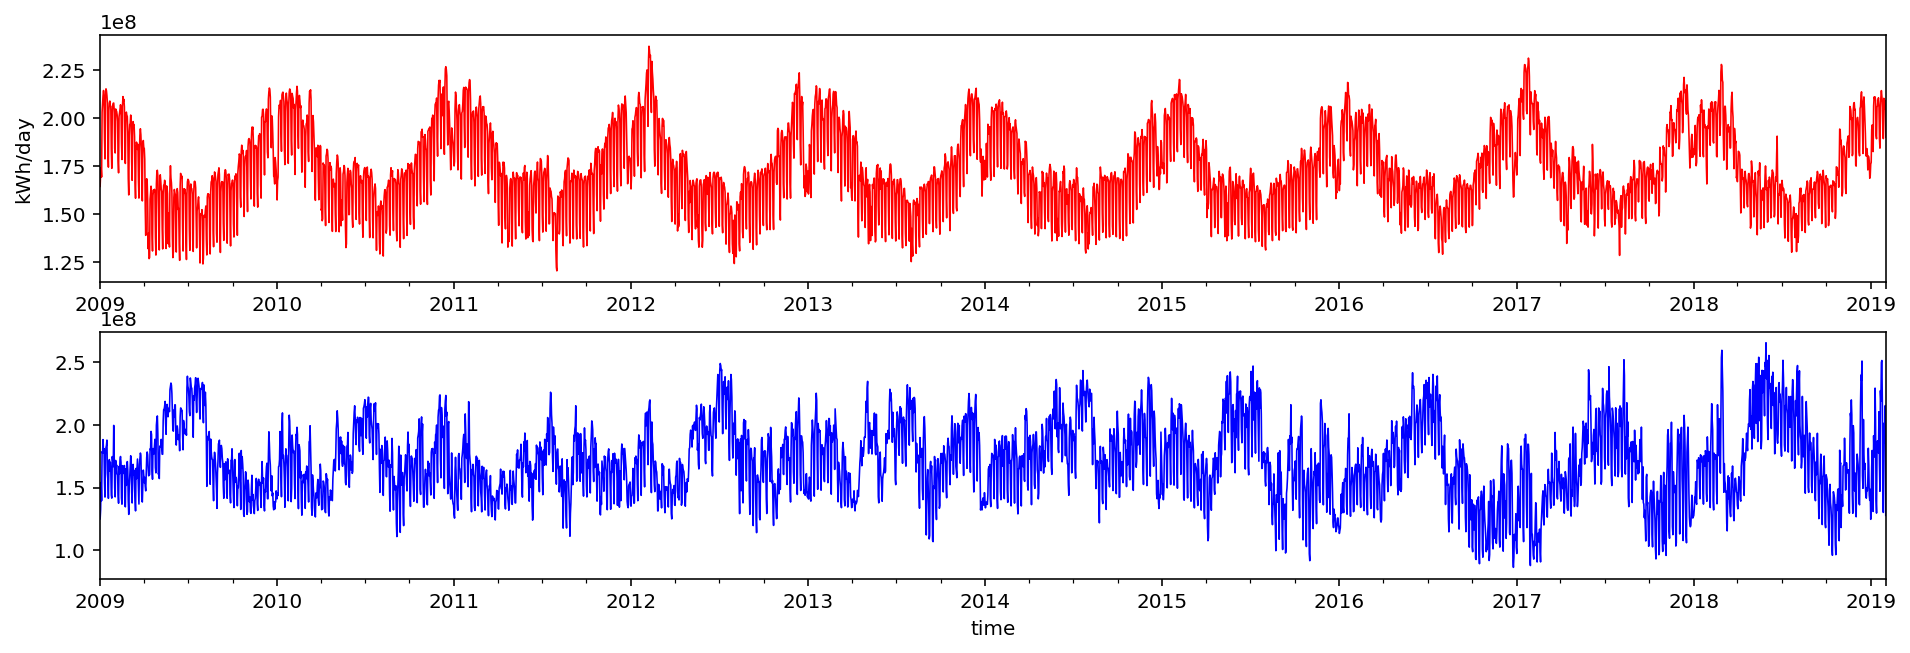
\includegraphics[width=\textwidth]{total_info.png}
    \caption{Daily energy consumption and production in Switzerland}
    \label{full dataset}
\end{figure}

\begin{figure}
    \centering
    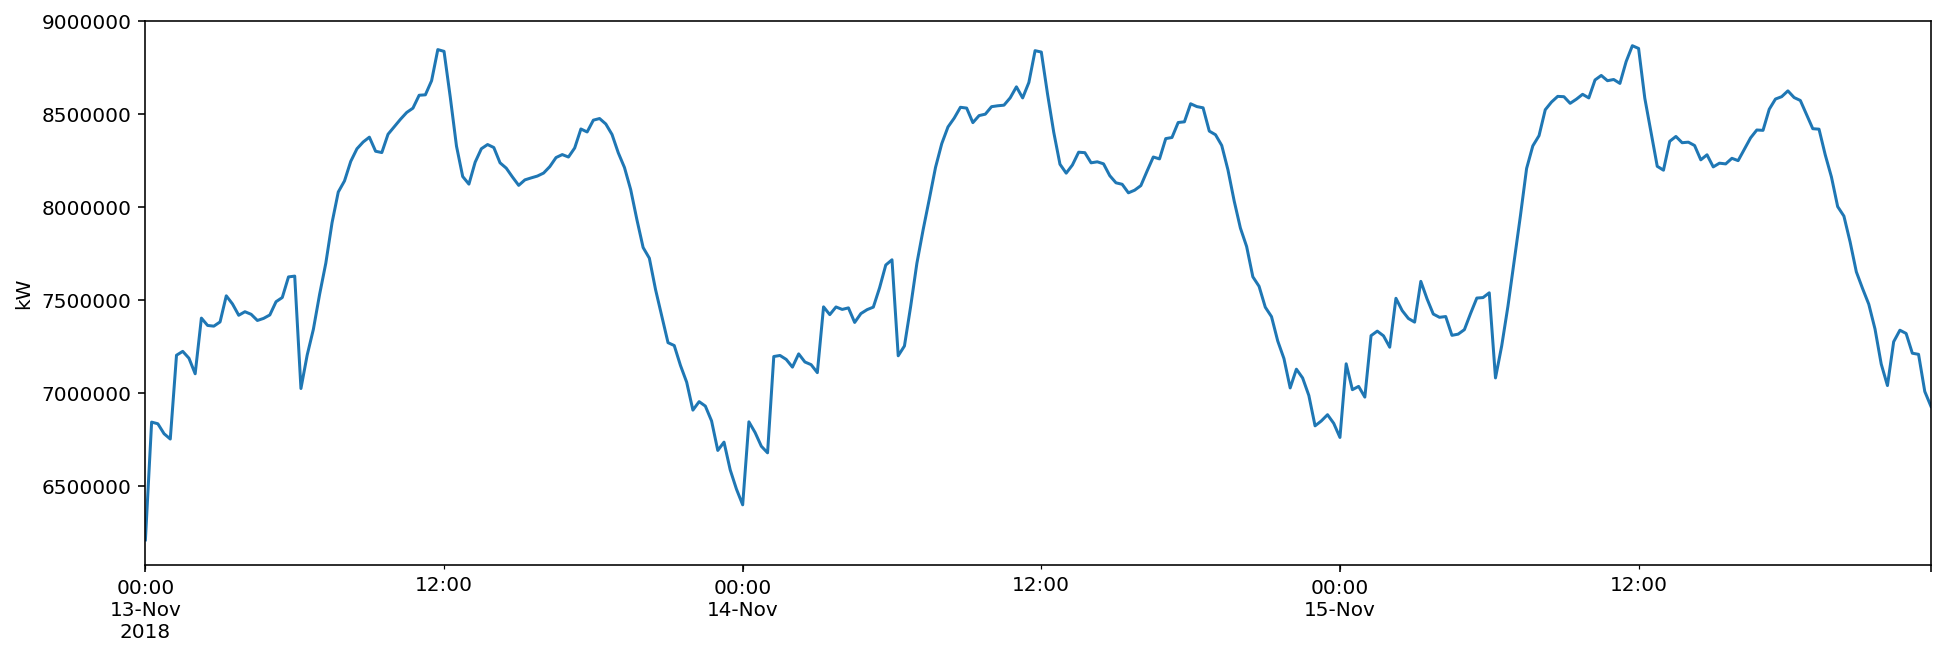
\includegraphics[width=\textwidth]{daily_seasonality.png}
    \caption{3 days of power consumption}
    \label{daily}
\end{figure}
\begin{figure}
    \centering
    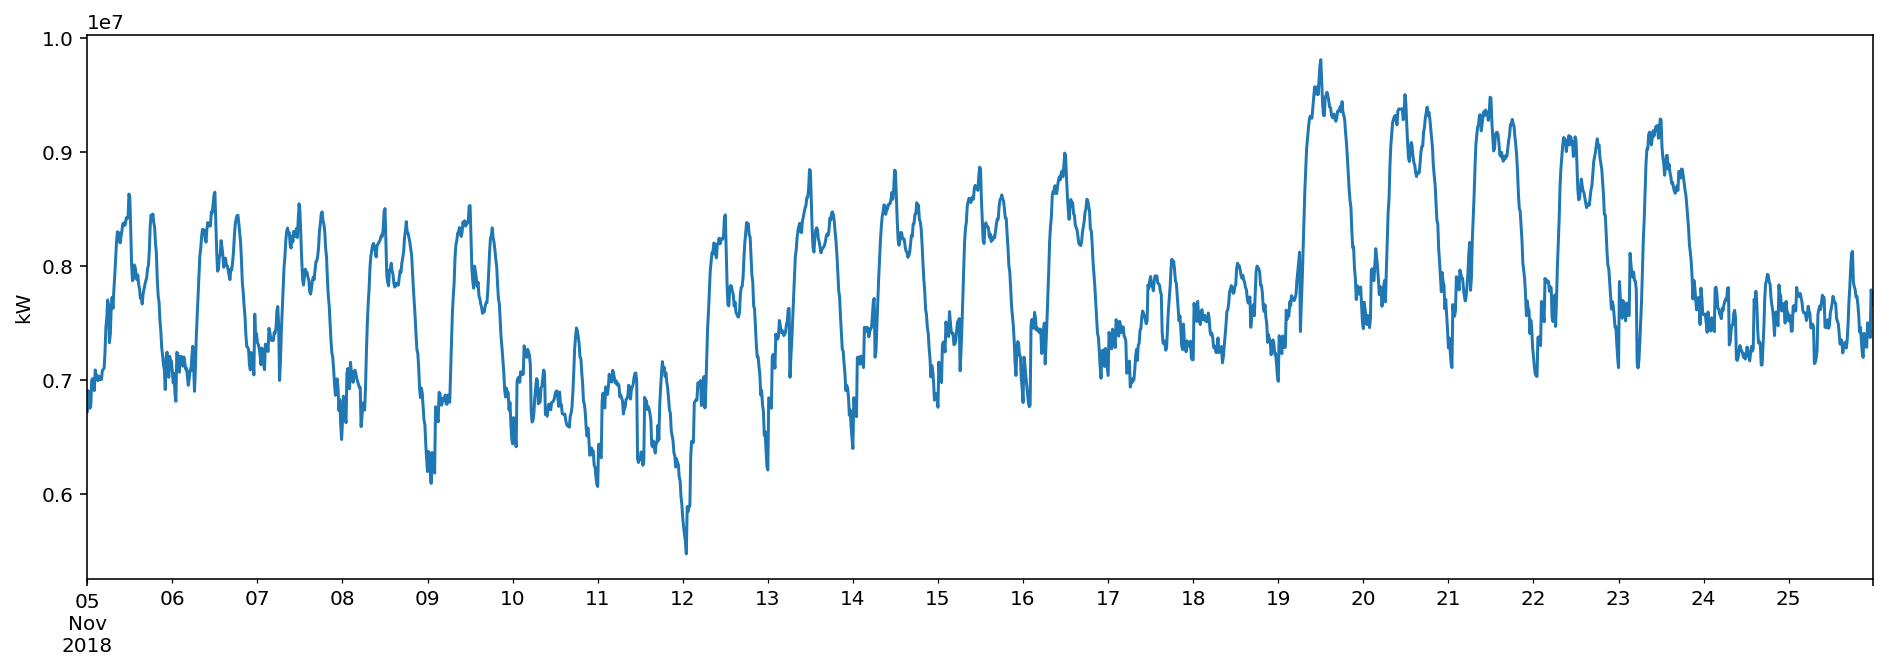
\includegraphics[width=\textwidth]{weekly_seasonality.png}
    \caption{3 weeks of power consumption}
    \label{weekly}
\end{figure}

\section{Aims and approach}
We anticipate that a big part of the work will deal with modeling the seasonal effects. Some of them have a precise periodicity, such as the 24 hours day cycle or the 7 day weekly ccycle, some other seasonal effects will require more attention: the exact date of the drop corresponding to easter holidays changes from year to year, and even festivities which happen at a fixed date, such as christmas, do not repeat at a completely regular pace, since some years count more days than others. A possible approach could be to introduce exogenous variables to represent holidays. We could eventually expand the model to account for the influence of weather variations on electrical demand.
Our final goal is to design a forecasting method for the consumption which could allow a controller of the power production facilities to minimize the difference between consumption and production.
As shown in figure \ref{rel_dif} at the moment the relative difference between the 2 quantities reaches some peaks of almost $80\%$. This might be a waste of money for the Swiss energy users, and also a damage for the environment since imported energy often comes from coal burning Germany.
Eventually, it could also be interesting to analyse the cantonal production/consumption in such a way to highlight how production could be tuned to minimize the losses due to energy transport between cantons.

\begin{figure}
    \centering
    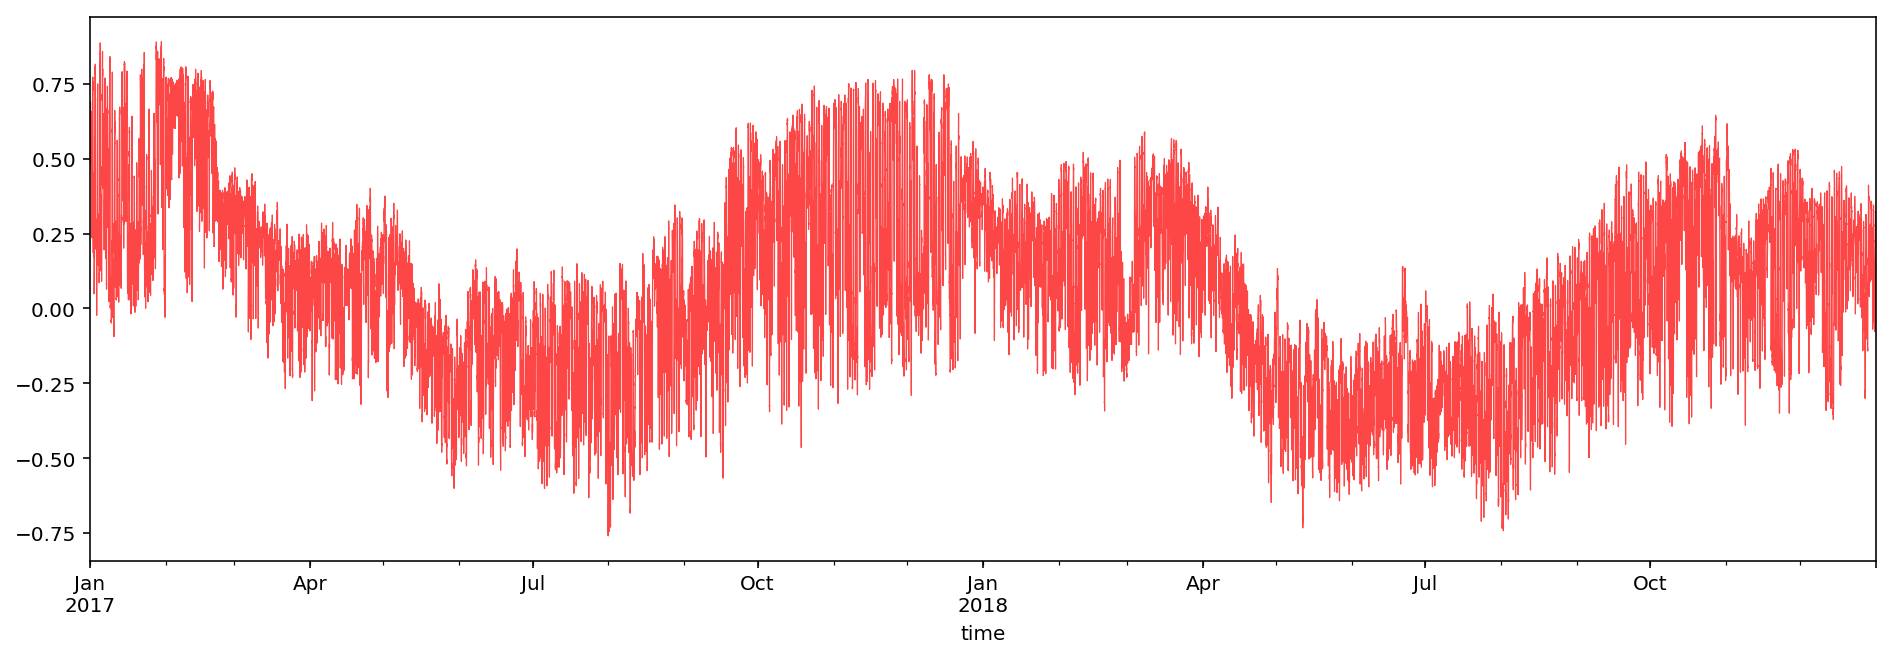
\includegraphics[width=\textwidth]{relative_difference.png}
    \caption{Relative difference between energy production and consumption computed as $d(a,b) = 2\frac{a-b}{a+b}$}
    \label{rel_dif}
\end{figure}


%-------------------------------------------------------------------------------
% REFERENCES
%-------------------------------------------------------------------------------
% \newpage
% \section*{References}

%[2]John W. Eaton, David Bateman, Sren Hauberg, Rik Wehbring (2015). GNU
%Octave version 4.0.0 manual: a high-level interactive language for numer-
%ical computations. Available: http://www.gnu.org/software/octave/doc/
%interpreter/. 
}
\end{document}

